\documentclass{standalone}
\usepackage{tikz}
\usetikzlibrary{patterns, positioning}


\begin{document}
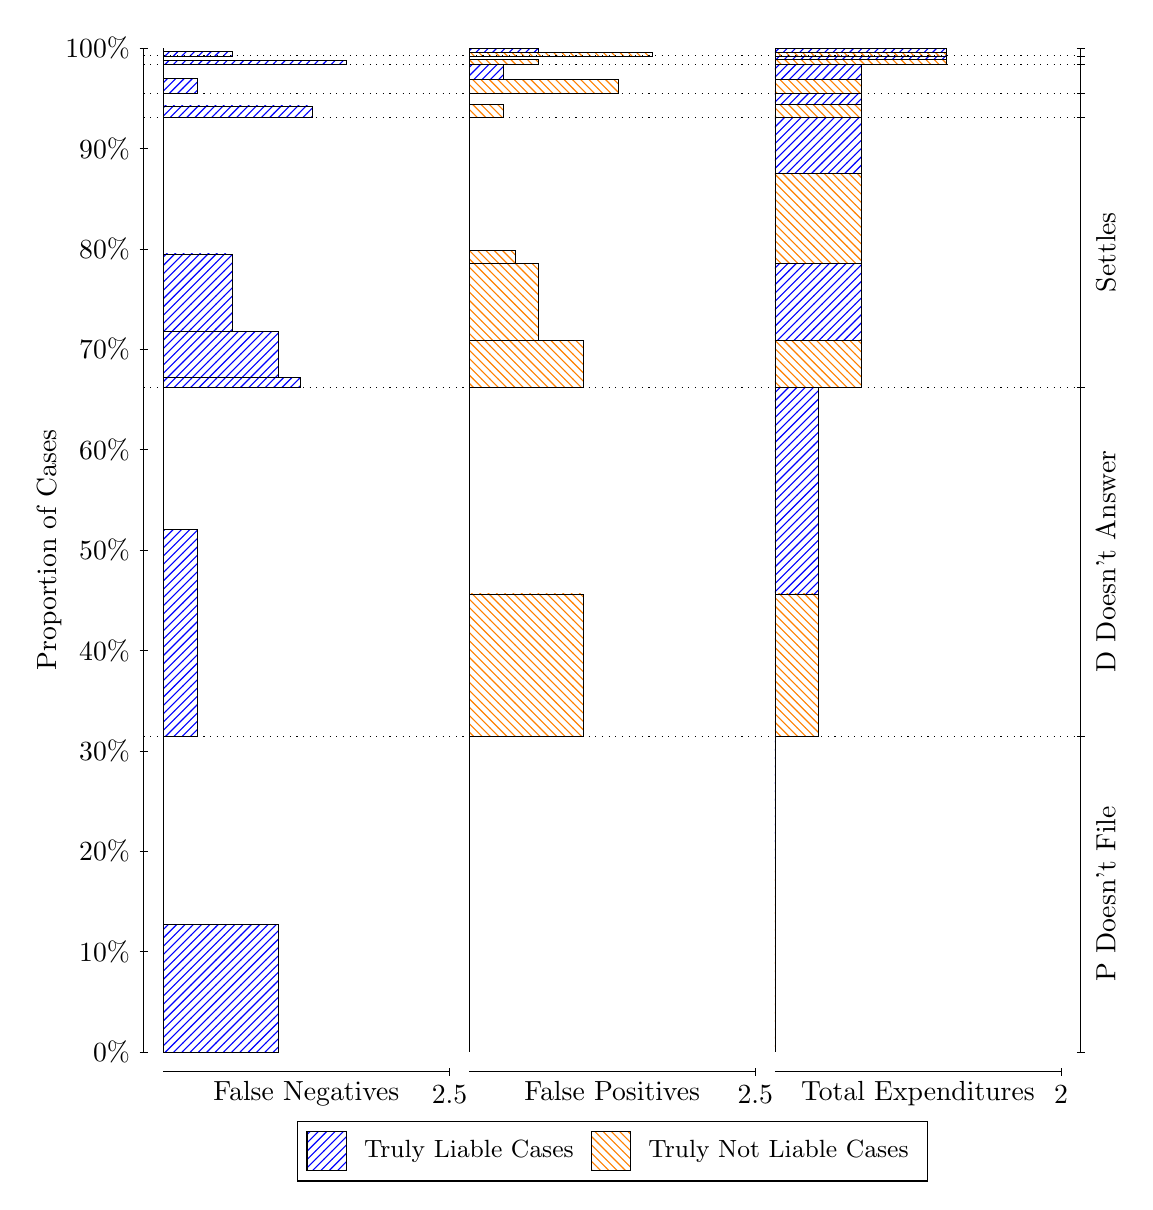
\begin{tikzpicture}
\draw[black, very thin] (1.5,1.75) -- (1.5,14.5);
\node[rotate=90, text=black, anchor=center] at (0.3, 8.125) {Proportion of Cases};
\draw[black, very thin] (1.45,1.75) -- (1.55,1.75);
\node[text=black, anchor=east] at (1.45, 1.75) {0\%};
\draw[black, very thin] (1.45,3.025) -- (1.55,3.025);
\node[text=black, anchor=east] at (1.45, 3.025) {10\%};
\draw[black, very thin] (1.45,4.3) -- (1.55,4.3);
\node[text=black, anchor=east] at (1.45, 4.3) {20\%};
\draw[black, very thin] (1.45,5.575) -- (1.55,5.575);
\node[text=black, anchor=east] at (1.45, 5.575) {30\%};
\draw[black, very thin] (1.45,6.85) -- (1.55,6.85);
\node[text=black, anchor=east] at (1.45, 6.85) {40\%};
\draw[black, very thin] (1.45,8.125) -- (1.55,8.125);
\node[text=black, anchor=east] at (1.45, 8.125) {50\%};
\draw[black, very thin] (1.45,9.4) -- (1.55,9.4);
\node[text=black, anchor=east] at (1.45, 9.4) {60\%};
\draw[black, very thin] (1.45,10.675) -- (1.55,10.675);
\node[text=black, anchor=east] at (1.45, 10.675) {70\%};
\draw[black, very thin] (1.45,11.95) -- (1.55,11.95);
\node[text=black, anchor=east] at (1.45, 11.95) {80\%};
\draw[black, very thin] (1.45,13.225) -- (1.55,13.225);
\node[text=black, anchor=east] at (1.45, 13.225) {90\%};
\draw[black, very thin] (1.45,14.5) -- (1.55,14.5);
\node[text=black, anchor=east] at (1.45, 14.5) {100\%};

\draw[black, very thin] (13.4,1.75) -- (13.4,14.5);
\draw[black, very thin] (13.35,1.75) -- (13.45,1.75);
\node[anchor=west] at (13.35, 1.75) {};
\draw[black, very thin] (13.35,5.762) -- (13.45,5.762);
\node[anchor=west] at (13.35, 5.762) {};
\draw[black, very thin] (13.35,10.194) -- (13.45,10.194);
\node[anchor=west] at (13.35, 10.194) {};
\draw[black, very thin] (13.35,13.623) -- (13.45,13.623);
\node[anchor=west] at (13.35, 13.623) {};
\draw[black, very thin] (13.35,13.928) -- (13.45,13.928);
\node[anchor=west] at (13.35, 13.928) {};
\draw[black, very thin] (13.35,14.294) -- (13.45,14.294);
\node[anchor=west] at (13.35, 14.294) {};
\draw[black, very thin] (13.35,14.401) -- (13.45,14.401);
\node[anchor=west] at (13.35, 14.401) {};
\draw[black, very thin] (13.35,14.5) -- (13.45,14.5);
\node[anchor=west] at (13.35, 14.5) {};

\draw[black, very thin, pattern color=blue, pattern=north east lines] (1.75,1.75) rectangle (3.2033,3.3719);
\draw[black, very thin, pattern color=orange, pattern=north west lines] (1.75,3.3719) rectangle (1.75,5.762);
\draw[black, very thin, pattern color=blue, pattern=north east lines] (1.75,5.762) rectangle (2.186,8.3876);
\draw[black, very thin, pattern color=orange, pattern=north west lines] (1.75,8.3876) rectangle (1.75,10.194);
\draw[black, very thin, pattern color=blue, pattern=north east lines] (1.75,10.194) rectangle (3.494,10.315);
\draw[black, very thin, pattern color=blue, pattern=north east lines] (1.75,10.315) rectangle (3.2033,10.906);
\draw[black, very thin, pattern color=blue, pattern=north east lines] (1.75,10.906) rectangle (2.622,11.886);
\draw[black, very thin, pattern color=orange, pattern=north west lines] (1.75,11.886) rectangle (1.75,13.623);
\draw[black, very thin, pattern color=blue, pattern=north east lines] (1.75,13.623) rectangle (3.6393,13.765);
\draw[black, very thin, pattern color=orange, pattern=north west lines] (1.75,13.765) rectangle (1.75,13.928);
\draw[black, very thin, pattern color=blue, pattern=north east lines] (1.75,13.928) rectangle (2.186,14.119);
\draw[black, very thin, pattern color=orange, pattern=north west lines] (1.75,14.119) rectangle (1.75,14.294);
\draw[black, very thin, pattern color=blue, pattern=north east lines] (1.75,14.294) rectangle (4.0753,14.341);
\draw[black, very thin, pattern color=orange, pattern=north west lines] (1.75,14.341) rectangle (1.75,14.401);
\draw[black, very thin, pattern color=blue, pattern=north east lines] (1.75,14.401) rectangle (2.622,14.456);
\draw[black, very thin, pattern color=orange, pattern=north west lines] (1.75,14.456) rectangle (1.75,14.5);
\draw[black, very thin, pattern color=orange, pattern=north west lines] (5.6333,1.75) rectangle (5.6333,4.1401);
\draw[black, very thin, pattern color=blue, pattern=north east lines] (5.6333,4.1401) rectangle (5.6333,5.762);
\draw[black, very thin, pattern color=orange, pattern=north west lines] (5.6333,5.762) rectangle (7.0867,7.5679);
\draw[black, very thin, pattern color=blue, pattern=north east lines] (5.6333,7.5679) rectangle (5.6333,10.194);
\draw[black, very thin, pattern color=orange, pattern=north west lines] (5.6333,10.194) rectangle (7.0867,10.784);
\draw[black, very thin, pattern color=orange, pattern=north west lines] (5.6333,10.784) rectangle (6.5053,11.765);
\draw[black, very thin, pattern color=orange, pattern=north west lines] (5.6333,11.765) rectangle (6.2147,11.93);
\draw[black, very thin, pattern color=blue, pattern=north east lines] (5.6333,11.93) rectangle (5.6333,13.623);
\draw[black, very thin, pattern color=orange, pattern=north west lines] (5.6333,13.623) rectangle (6.0693,13.785);
\draw[black, very thin, pattern color=blue, pattern=north east lines] (5.6333,13.785) rectangle (5.6333,13.928);
\draw[black, very thin, pattern color=orange, pattern=north west lines] (5.6333,13.928) rectangle (7.5227,14.104);
\draw[black, very thin, pattern color=blue, pattern=north east lines] (5.6333,14.104) rectangle (6.0693,14.294);
\draw[black, very thin, pattern color=orange, pattern=north west lines] (5.6333,14.294) rectangle (6.5053,14.354);
\draw[black, very thin, pattern color=blue, pattern=north east lines] (5.6333,14.354) rectangle (5.6333,14.401);
\draw[black, very thin, pattern color=orange, pattern=north west lines] (5.6333,14.401) rectangle (7.9587,14.445);
\draw[black, very thin, pattern color=blue, pattern=north east lines] (5.6333,14.445) rectangle (6.5053,14.5);
\draw[black, very thin, pattern color=orange, pattern=north west lines] (9.5167,1.75) rectangle (9.5167,4.1401);
\draw[black, very thin, pattern color=blue, pattern=north east lines] (9.5167,4.1401) rectangle (9.5167,5.762);
\draw[black, very thin, pattern color=orange, pattern=north west lines] (9.5167,5.762) rectangle (10.062,7.5679);
\draw[black, very thin, pattern color=blue, pattern=north east lines] (9.5167,7.5679) rectangle (10.062,10.194);
\draw[black, very thin, pattern color=orange, pattern=north west lines] (9.5167,10.194) rectangle (10.607,10.784);
\draw[black, very thin, pattern color=blue, pattern=north east lines] (9.5167,10.784) rectangle (10.607,11.765);
\draw[black, very thin, pattern color=orange, pattern=north west lines] (9.5167,11.765) rectangle (10.607,12.91);
\draw[black, very thin, pattern color=blue, pattern=north east lines] (9.5167,12.91) rectangle (10.607,13.623);
\draw[black, very thin, pattern color=orange, pattern=north west lines] (9.5167,13.623) rectangle (10.607,13.785);
\draw[black, very thin, pattern color=blue, pattern=north east lines] (9.5167,13.785) rectangle (10.607,13.928);
\draw[black, very thin, pattern color=orange, pattern=north west lines] (9.5167,13.928) rectangle (10.607,14.104);
\draw[black, very thin, pattern color=blue, pattern=north east lines] (9.5167,14.104) rectangle (10.607,14.294);
\draw[black, very thin, pattern color=orange, pattern=north west lines] (9.5167,14.294) rectangle (11.697,14.354);
\draw[black, very thin, pattern color=blue, pattern=north east lines] (9.5167,14.354) rectangle (11.697,14.401);
\draw[black, very thin, pattern color=orange, pattern=north west lines] (9.5167,14.401) rectangle (11.697,14.445);
\draw[black, very thin, pattern color=blue, pattern=north east lines] (9.5167,14.445) rectangle (11.697,14.5);
\draw[black, dotted] (1.5,5.762) -- (13.4,5.762);
\draw[black, dotted] (1.5,10.194) -- (13.4,10.194);
\draw[black, dotted] (1.5,13.623) -- (13.4,13.623);
\draw[black, dotted] (1.5,13.928) -- (13.4,13.928);
\draw[black, dotted] (1.5,14.294) -- (13.4,14.294);
\draw[black, dotted] (1.5,14.401) -- (13.4,14.401);
\draw[black, very thin] (1.75,1.5) -- (5.3833,1.5);
\node[text=black, anchor=north] at (3.5667, 1.5) {False Negatives};
\draw[black, very thin] (5.3833,1.45) -- (5.3833,1.55);
\node[text=black, anchor=north] at (5.3833, 1.45) {2.5};

\draw[black, very thin] (5.6333,1.5) -- (9.2667,1.5);
\node[text=black, anchor=north] at (7.45, 1.5) {False Positives};
\draw[black, very thin] (9.2667,1.45) -- (9.2667,1.55);
\node[text=black, anchor=north] at (9.2667, 1.45) {2.5};

\draw[black, very thin] (9.5167,1.5) -- (13.15,1.5);
\node[text=black, anchor=north] at (11.333, 1.5) {Total Expenditures};
\draw[black, very thin] (13.15,1.45) -- (13.15,1.55);
\node[text=black, anchor=north] at (13.15, 1.45) {2};

\node[text=black, centered, rotate=90] at (13.72, 3.756) {P Doesn't File};
\node[text=black, centered, rotate=90] at (13.72, 7.9778) {D Doesn't Answer};
\node[text=black, centered, rotate=90] at (13.72, 11.908) {Settles};





\draw (7.449999999999999,1.5) node[draw=none] (baseCoordinate) {};
\begin{scope}[align=center]
        \matrix[scale=0.5, draw=black, below=0.5cm of baseCoordinate, nodes={draw}, column sep=0.1cm]{
            \node[rectangle, draw, minimum width=0.5cm, minimum height=0.5cm, pattern color=blue, pattern=north east lines] {}; &
            \node[draw=none, font=\small, text=black] (B) {Truly Liable Cases}; &
            \node[rectangle, draw, minimum width=0.5cm, minimum height=0.5cm, pattern color=orange, pattern=north west lines] {}; &
            \node[draw=none, font=\small, text=black] (B) {Truly Not Liable Cases}; \\
            };
\end{scope}

\end{tikzpicture}
\end{document}